\paragraph{Descarga de alimentos de la unidad de transporte}\label{sec:DescargaAlimentos}\index{Instrucción!descarga de alimentos de la unidad de transporte}

\begin{enumerate}
    \item Se hace la inspección de la unidad de transporte previo a comenzar a descargar el alimento;
    \item Se \emph{enrampa} la unidad y se abre la cortina del andén.
    \item Se inspeccionan los alimentos conforme a los criterios establecidos de acuerdo a si son:
        \begin{enumerate}
            \item alimentos congelados (ver \cref{esp.crit.acep-cong});
            \item alimentos refrigerados (ver \cref{esp.crit.acep-refri});
            \item alimentos de almacenamiento especial.
        \end{enumerate}
        \begin{itemize}
            \item[\textbf{Si no cumple}] si la temperatura del alimento excede los criterios establecidos para el tipo de almacenamiento, se rechaza la unidad.
        \end{itemize}
    \item Si el alimento viene sobre tarimas, este se descarga de la unidad y se dispone en el andén para que el \emph{personal de embarques} tome nota de la mercancía que se está descargando para posteriormente ingresarla en el \gls{SGA}.
    \begin{enumerate}
        \item En caso de que el \emph{alimento entarimado} requiera de descopete:\\
        se armarán las tarimas adicionales, cuidando el no mezclar lotes diferentes.
        \item En caso de que las tarimas del \emph{alimento entarimado} esten en malas condiciones:\\
        \begin{enumerate}
            \item Si la tarima se puede cargar sin romperse:
                \begin{itemize}
                    \item Se colocará la tarima en malas condiciones sobre una tarima nueva y se cobrará(n) la(s) empleadas.
                    \item Esta accion tiene que registrarse en el \Oent.
                \end{itemize}
            \item Si la tarima viene en muy malas condiciones o si el cargar la tarima podria significar un \gls{peligro-relacionado-con-la-inocuidad-de-los-alimentos}:
                \begin{itemize}
                    \item Se armará una tarima nueva manualmente
                    \item Esta accion tiene que registrarse en el \Oent.
                    \item Se cobrará por armado de tarima y por venta de tarima.
                \end{itemize}
        \end{enumerate}
    \end{enumerate}
    \item Se etiquetarán las tarimas descargadas:\\
    Posterior al ingreso de los datos al \gls{SGA}, {\itshape\MC} genera las etiquetas correspondientes para las tarimas a almacenar. Estas se deben de poner de manera que sean visibles, entre el material de emplaye.
    \item Se almacenarán los alimentos en la cámara correspondiente.
\end{enumerate}

\begin{scheme}[p]
    \centering
    % \missingfigure[figheight=0.9\textheight]{Diagrama sobre descarga de alimentos}
    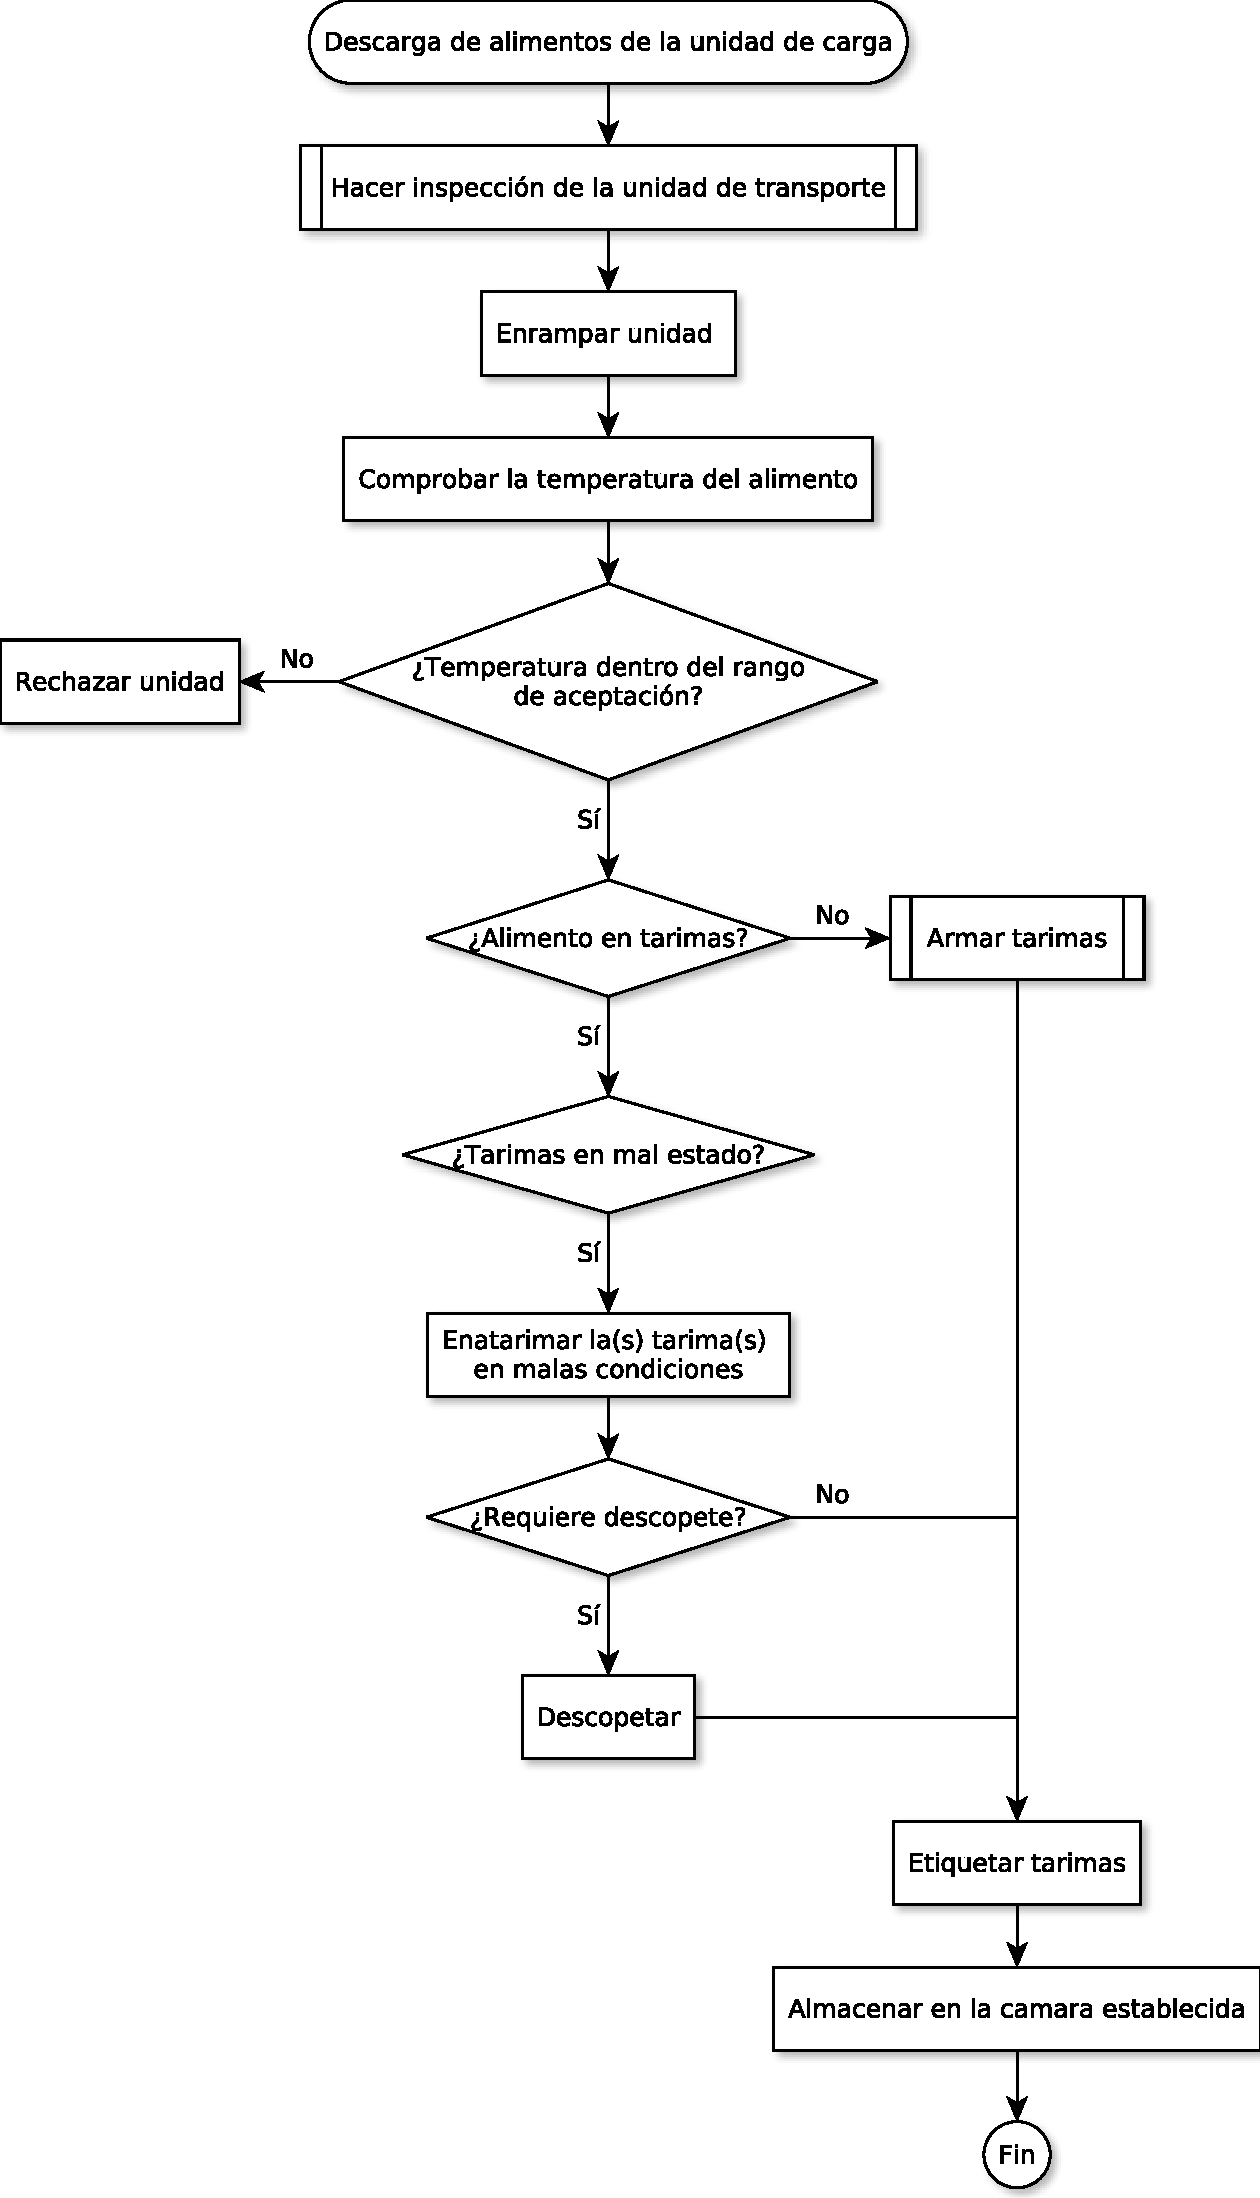
\includegraphics[height=0.9\textheight]{../IT/IT-2.pdf}
    \caption[Proceso de descarga de unidades posterior a la inspección]{Proceso de descarga de unidades posterior a la inspección. Para mayor información, consultar el \cref{sec:DescargaAlimentos}.}
\end{scheme}

\clearpage